%tapered_waveguide
Tapered waveguide is composed of a regular waveguide and a taper interface, whose dimensions in the tapered section changes slightly along the longitudinal direction\cite{linear_tapered_waveguides}. Tapered structure enables the waveguide to receive more light so that this structure can improve the coupling efficiency between beam source and waveguide.\\  

\begin{figure}[!ht]
\centering
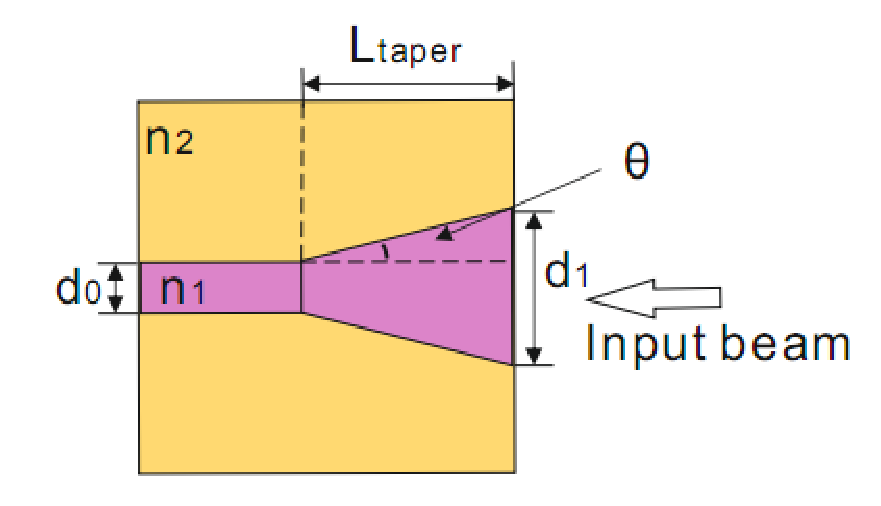
\includegraphics[width=0.7\textwidth]{bilder/convernational_taper}
\caption{Schema of a conventional taper.}
\label{fig:conventional_taper}
\end{figure}
%\begin{figure}[!ht]
%\centering
%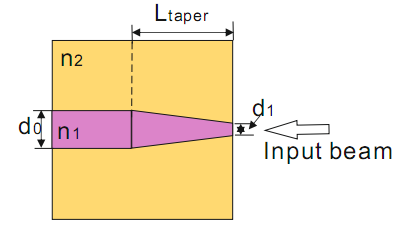
\includegraphics[width=0.7\textwidth]{bilder/inverse_taper}
%\caption{Schema of a inverse taper.}
%\label{fig:inverse_taper}
%\end{figure}
Nathaniel in \cite{design_fabrication_tapered_waveguide} has presented two general types of tapered waveguide: conventional taper like Fig. \ref{fig:conventional_taper} and inverse taper. For a conventional taper the entry is wider than the exit, while for an inverse taper the entry is narrower than the exit. Because the entry of the inverse taper has smaller dimensions than that of beam spots in this work, only the conventional taper will be discussed in this section.\\

In this section only the simple taper structure is involved for considering the fabrication process of a rib waveguide. Therefore only two taper properties, the width $d_{1}$ of a taper interface and the divergence angle $\theta$ of the taper, are discussed. For convenient calculations simulations in this section will be arranged respectively due to variations of taper width and taper length $L_{taper}$.
